\scanpage{67}
% archive foliation: 66
\diagram{\begin{tabular}{c l}
U N I V E R S I T E & Montpellier, le 28 Juin 1978\\
DES SCIENCES ET TECHNIQUES &\\
DU LANGUEDOC &\\
\texttt{------------}&\\
Service de la Scolarité &\\
MR / GJ &\\
Diffusion : Liste A &\\
N° : 4066 &
\end{tabular}}
\uline{AVIS DE SOUTENANCE D'UNE THESE DE DOCTORAT DE 3ème CYCLE}

\uline{( CHIMIE ORGANIQUE PHYSIQUE )}

\uline{Nom et prénom du candidat} :\qquad AURELLY Michèle

\uline{Titre de la thèse} : Application de la corrélation de Hammett à l'étude de l'énolisation des cétones en milieux basique et superbasique.

\uline{Date, heure et lieu de soutenance prévus} :

JEUDI 13 JUILLET 1978 à 16 Heures\\
Salle de cours n° 9 - U. S. T. L.

\uline{Nom du Directeur de thèse} :

Monsieur le Professeur LAMATY.

\uline{Désignation du laboratoire où la thèse est préparée} :

Laboratoire de Chimie Organique Physique.

\uline{Analyse de l'ouvrage} :

Ce travail consiste à cerner de plus près les mécanismes de l'énolisation des cétones par l'étude d'acétophénones et de méthyl-2 phényl-1 butanones-1 substituées, dans des milieux basiques. Les constantes p de Hammett ont été mesurées en fonction de la nature du milieu.

\uline{Durée approximative des recherches ayant abouti à la thèse : 3 ans.}

\uline{Composition du jury proposé} :
\diagram{\begin{tabular}{ll}
MM. : & LAMATY, Président\\
& SCHUE\\
& WYLDE\\
& MION
\end{tabular}}
Le Secrétaire Général,

\figure{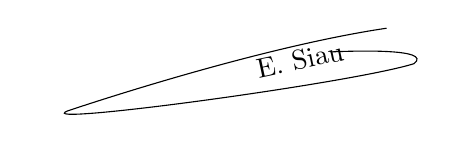
\begin{tikzpicture}[x=1cm,y=1cm]
\node[rotate=12] at (1.55,.25){\unsure{E. Siau}};
\draw (2.65,.65) .. controls (1.3,.45) and (-.5,-.1) .. (-1.4,-.4)
.. controls (-1.9,-.6) and (2.2,-.05) .. (3,.2)
.. controls (3.25,.4) and (2.2,.36) .. (1.96,.35);
\end{tikzpicture}}

\uline{E. SIAU}
